I dette kapittelet ønsker vi å utrede hvordan vi gjennomførte hvert steg av forskningsplanen Kapittel \ref{chap:fremgangsmate}. De påfølgende underkapitlene er litteratursøk, utvikling av prototype og gjennomføring av eksperimentet.
\section{Litteratursøk}
Et litteratursøk ble foretatt for å se hva som er gjort tidligere i vårt problemdomene. Litteratursøk innebærer å finne kunnskap tilgjengelig i forskjellige databaser, for å kritisk gjennomgå disse. Siden vårt problemdomene går inn på flere fagområder, valgte vi å dele inn litteratursøket i flere deler. Siden planen er å utvikle et støtteverktøy med semantisk webteknologi der brukeren utfører legemiddelgjennomgang, ble inndelingen følgende: 1)Hvilken informasjon trenger helsepersonnell ved legemiddelgjennomgang 2)Forsøk på beslutningsstøtte til legemiddelgjennomgang eller forskrivning av legemidler 3)Bruk av semantisk webteknologi for modellering av legemiddelinformasjon. Databasene vi tok i bruk for å finne litteratur for disse temaene var hovedsakelig PubMed og Google Scholar. IEEE Xplore, UpToDate og Tidsskriftet.no ble brukt i mindre grad.              
\label{chap:gjenomf_litteratursok}
\subsection{Behov for legemiddelinformasjon}
Vår prototype skal forsøke å gi kliniske farmasøyter tilstrekkelig informasjon om legemidler. Derfor har vi foretatt et litteratursøk for å se på helsepersonells behov for legemiddelinformasjon ved behandling av pasienter.

Hvilke faktorer som påvirker helsepersonells valg av kilder er uklart. I en hektisk arbeidshverdag der tiden er knapp viser det seg at man i primærhelsetjenesten setter effektivitet høyt når det gjelder valg av kilder \citep{Cook_Sorensen_2013}. Med effektivitet menes at kilden har svaret på det kliniske spørsmålet de lurer på, og at det er enkelt å finne fram til svaret. Hvor raskt man kan finne svaret er avhengig av struktur av kilden, søkefunksjonalitet, lengde på innhold og kjennskap til bruken. Videre er det andre faktorer som spiller inn på valg av kilder som inkluderer tett integrasjon i arbeidsflyten, kredibilitet, kontaktinfo til ekspert, rettet mot kliniske spørsmål, oversettelse til lokale behandlingsprosesser og mulighet for pasientopplæring. Ingen av kildene nevnt, blant annet PubMed, MEDLINE og UpToDate, dekker alle behovene.

Fastleger har behov for legemiddelinformasjon til støtte under forskrivning, men informasjonen gitt av beslutningsstøttesystemer møter ofte ikke deres behov\citep{Rahmner_Eiermann_2012}. Interaksjoner, bivirkninger, allergier og hypersensitivitet, aldersrelatert dosering og indikasjoner var noen av informasjonsbehovene som ble nevnt. Flere rapporterte eksempelvis at interaksjoner var oppgitt i beslutningsstøttesystemet i bruk, men at for mye informasjon gjorde at advarslene ble sett på som mindre viktige eller ignorert.  Ved aldersrelatert dosering var det ønske om at et system beregnet glomerulær filtrasjonsrate, slik at en kan enklere foreta riktige dosejusteringer for pasienter med nedsatt nyrefunksjon. 
\subsection{Klinisk beslutningsstøtte}
Prototypen er et forsøk på å undersøke hvorvidt støttesystem kan hjelpe kliniske farmasøyter i å utføre legemiddelgjennomganger. Et litteratursøk er derfor foretatt for å se på tidligere forskning omkring beslutningsstøtte for legemiddelgjennomgang og forskrivning av legemidler.
\subsubsection{STRIP}\label{STRIP}
Systematic Tool to Reduce Inappropiate Prescribing(STRIP) er et klinisk beslutningsstøttesystem for legemiddelgjennomgang utviklet i Nederland \citep{STRIP}. Verktøyet er beregnet for bruk i polyfarmasi, altså for pasienter som benytter flere medikamenter og i større doser enn ønskelig. STRIP tar i bruk og kombinerer START og STOPP-kriteriene for å gi ut en farmakoterapeutisk analyse som blant annet inkluderer sjekker for dosejustering, overbehandling og underbehandling, bivirkninger, interaksjoner, dosefrekvens og inntaksmåte. I tillegg til denne analysen tar STRIP også hensyn til pasientens preferanser og legemiddelhistorikk. Et eksperimentet viste at legemiddelgjennomgangen ble mer korrekt, altså at det ble gjort flere riktige avgjørelser og færre uriktige. På en annen side brukte de signifikant lengre tid på legemiddelgjennomgangen. Brukergrensesnittet var lite tilfredstillende i bruk. 

\subsubsection{SMART}
En nylig foretatt studie så på muligheten til å bedre legemiddelbehandlingen hos geriatrikere ved å implementere Beers kriterier og beregning av glomerulær filtrasjonsrate i et eksisterende EPJ-system\citep{SMART}. Denne beslutningsstøtten ble kalt Seniors Medication Alert and Review Technologies(SMART). SMART ga beslutningsstøtte enten passivt i form av meldinger i pasientjournalen(passiv støtte) eller advarsler ved dokumentering av legemidler(aktiv støtte). Denne støtten kunne avdekke uhensiktsmessige legemidler, nedsatt glomerulær filtrasjonsrate(GFR) samt dosejusteringer. GFR ble beregnet ut i fra høyde, vekt og kreatinin-nivåer klinikerne selv skrev inn i systemet. Hver enkelt anbefaling hadde en indikator som viste styrken på anbefalingen og  kvaliteten på evidens, samt lenker til læringsressurser og oppsummeringen av evidensen. Studien viste at klinikerne var enige om at SMART var tilfredstillende i bruk uten å legge store hindringer i arbeidsflyten. Advarslene ble brukt som læringsverktøy og benyttet som evidensbasert støtte ved beslutningstaking. Videre mente klinikerne at SMART styrket, og i noen tilfeller endret deres kliniske beslutning.
\subsubsection{Renal beslutningsstøtte i Janus pasientjournal}
Janusinfo er et pasientjournalsystem med tilhørende verktøy i Sverige.
\ot{Si noe om dette Janus pasientjournalsystemet?}

The Renal Button er navnet på en pilot av et beslutningsstøttesystem ment for å støtte dosering av legemidler basert på en estimering pasienters utskillelse av kreatinin\citep{Hellden_Al-Aieshy_2015}. Renal utskillelse av legemidler er korrelert til utskillelse av kreatinin. Beslutningsstøtten ble implementert i Janus pasientjournalsystem. The Renal Button ga støtte svar på 1)Er legemiddelet hensiktsmessig og hvilken dosering,2)Risikoen for å ikke tilpasse dosen etter evne til utskillelse av kreatinin. Hvert forslag inkluderte en større tekstlig beskrivelse samt referering til kilder. Estimasjon av kreatininnivå ble beregnet ved å bruke pasientdata som alder, kroppsvekt, kjønn og P-kreatinin hentet fra informasjonen i EPJ-systemet. En evaluering av systemet undersøkte pilotens nytteverdi og brukernes oppfattelse av brukergrensesnittet. Samtidig ble antall pasienter med estimert utskillelse av kreatinin før og etter bruk av systemet målt. Antall pasienter med estimert utskillelse av kreatinin økte med 1.6 etter bruk av systemet.

Et annet pilotprosjekt utviklet et beslutningsstøttesystem for forskrivning av legemidler til pasienter med nedsatt nyrefunksjon\citep{Shemeikka_Bastholm-Rahmner_2015}. Dette ble også implementert i Janus pasientjournalsystem. Istedenfor å estimere utskillelse av kreatinin, ble estimert glomerulær filtrasjonsrate(eGFR) brukt for dosejustering etter pasientens nyrefunksjon. Verdien av eGFR ble vist sammen med legemiddellisten. Systemet ga anbefalinger for dose, som var klassifisert etter hvorvidt nedsatt nyrefunksjon påvirket pasientens opptak av legemiddelet. Evaluering av beslutningsstøttesystemet viste at deltagerne fikk økt forståelse for dosering, og at bruken av støtten var tidsbesparende.   

\subsection{Semantisk modellering av legemiddelkunnskap}
Prototypen skal bruke semantisk webteknologi for å modellere legemiddelkunnskap. Denne seksjonen utgreier om tidligere arbeid og forskning på modellering av legemiddelkunnskap og tilhørende informasjon med semantiske webteknologier.

\subsubsection{Modellering av farmakogenetikk}
En studie beskriver et pilotprosjekt der målet var å bygge en semantisk modell av farmakogenetisk informasjon knyttet til legemidler\citep{Boyce_Freimuth_2013}. Formålet med å bygge en slik modell var å bruke strukturert farmakogenetisk informasjon som beslutningsstøtte i klinisk-og-translasjonsforskning. Beslutningsstøtten skulle svare på spesifikke kliniske spørsmål, f.eks: For pasient med genotype x, finn anbefaling for et legemiddel, inkludert doseendringer og eventuelt alternative legemidler. 

\subsubsection{Open PHACTS}
Open pharmacological concepts triple store (open PHACTS) er en platform ment for å assistere funn av potensielle legemidler. Ved bruk av semantisk webteknologi, er datagrunnlaget satt sammen av flere heterogene informasjonskilder forskere innenfor farmakologi, medisin og bioteknologi allerede bruker. Disse kildene inneholder detaljert farmakologisk informasjon om legemidler, stoffer, molekylære forbindelser, kjemisk strukturer, enzymer, gener, reaksjonsveier og mer. Tjenesten brukes enten som et webgrensesnitt eller ved bruk av et API\citep{open_phacts_explorer}. En studie har sett på hvordan Open PHACTS kan støtte funn av potensielle legemidler\citep{Ratnam_2014}. Videre konkluderer studien med at Open PHACTS løser tidligere integrasjonsproblemer den enkelte hadde i form av lisensiering, formattering og søk.

\subsubsection{DrOn}
\gls{dron} er en modulær ontologi for legemiddel-produkter utviklet med semantiske teknologier. Den innehar informasjon om ingredienser og biologisk aktivitet med utgangspunkt i legemidler som selges i USA \citep{dron_2013}. Ontologien bruker RxNorm som dets eksterne hovedkilde, som er en medisinsk terminologi som inneholder alle legemidler til salgs i USA. Disse legemidlene er kartlagt opp mot ChEBI-klasser. \gls{chebi} er en database og ontologi som inneholder molekylære entiteter. Resultat av dette er at en kan resonnere mellom legemidler med tilhørende ingredienser og biologiske aktivitet. 

For å lage denne ontologien minet de data fra utgivelser av RxNorm. Dette ble gjort ved å laste ned råfilene, omforme dataene for å deretter importere dette i en relasjonsdatabase ved hjelp av et skript som er tilgjengelig. Så ble RxNorm-entiteter kartlagt opp mot ChEBI-klasser ved hjelp av en konsollapplikasjon som sammenlignet etiketter av ingredienser i RxNorm med klasseannoteringer i \gls{chebi}. Deretter ble den normaliserte databasen oversatt til en OWL-artefakt. 

\gls{dron} er modulært, slik at klasser fra hver kilde er serialisert i separate moduler som igjen er konsumert(del av..) av klasser som er manuelt utarbeidet på et høyere nivå i en modul med termer som «klinisk rolle», «tablett», «kapsel» med mer. På denne måten kan en enkelt bruke deler av ontologien i tillegg til at videreutvikling vil være enklere. 

Denne ontologien inneholder mye informasjon om legemidler, og kan spille en viktig rolle i utviklingen av vårt system. Framgangsmåten deres kan være nyttig for oss, selv om vi velger å ikke ta i bruk \gls{dron}. Hvis vi går for å bruke \gls{dron} på en eller annen måte, er det visse aspekter med ontologien vi må ta stilling til. Den største problemstillingen vil nok være å bruke denne ontologien i norsk sammenheng. Er det mulig å koble amerikanske legemidler opp mot legemidler til salgs i Norge? 
\section{Utvikling av prototype}
I følgende underkapitler vil vi legge frem bakgrunnen og oversikten, totaldesign og dermed bryte opp totalen for å legge frem hvordan vi har designet de forskjellige delene. Vi vil også vise en liten demostrasjon av hvordan prototypen så ut og hvordan vi gjennomførte forsøket med prototypen. Dette underkapitelet vil være teknisk og vil vise teknologiske valg som ble tatt underveis.
\label{chap:gjenomf_utviklingavprototype}
\subsection{Bakgrunn}

Semantisk legemiddelgjennomgang (SemLMG) var en prototype som ble utviklet hvor formålet var et støtteverktøy under legemiddelgjennomgang. Prototypen skulle gi brukeren relevant og enkelt tilgjengelige tiltak for legemidler for å se om den kunne gi et bedre beslutningsgrunnlag. For å kunne realisere prototypen ville prototypen foreslå tiltak for en bestemt kategori under legemiddelgjennomgangen. Kategorien heter ''Legemiddel ikke tilpasset pasient''. Denne kategorien går på tiltak for nyre- og leverfunksjoner. Tiltakene som prototypen presenterte for brukeren var tiltak ved nedsatt nyrefunksjon.

En bruker skal kunne lese en kasuistikk, få en oversiktlig liste over legemidler og til slutt få opp et skjema som brukes til å utføre en legemiddelgjennomgang. Prototypen var designet slik at noen varianter av kasuistikkene var med eller uten foreslåtte tiltak. Prototypen skulle brukes når og hvor som helst i en bestemt tidsperiode.

%Brukere av prototypen var kliniske farmasøyter som skulle lese en kasuistikk, observere at en samstemt liste blir laget og dermed utføre en legemiddelgjennomgang. Utførelsen av legemiddelgjennomgangen skulle utføres på vanlig vis med vår prototype. Med vanlig vis mener vi at brukerene skulle gjøre legemiddelgjennomgangen så likt virkeligheten som mulig. Dette vil bety at farmasøytene brukte eksterne kilder for å foreslå tiltak. Prototypen var designet slik at noen varianter av kasuistikkene var med eller uten foreslåtte tiltak. For å kunne måle hvor lang tid brukerene bruker under de forskjellige stegene av prototypen ble det gjort tidsmåling i hvert steg. Prototypen var ønsket å kunne brukes når og hvor som helst i en bestemt tidsperiode.
\subsection{Use-case diagram}
Under utvikling av prototypen var det viktig å ha definert en rolle og handlingene mellom rollen og systemet. For å holde oversikt og fokus modellerte vi et use-case diagram (Figur \ref{fig:ucd}
\begin{figure}[H]
\centering
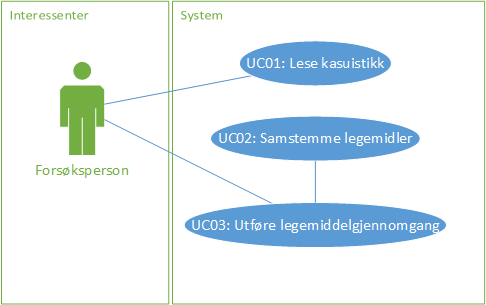
\includegraphics[width=14cm]{images/ucd.png}
\caption{Use-case diagram}
\label{fig:ucd}
\end{figure}
\subsubsection{UC01: Lese kasuistikk}
En forsøksperson skulle kunne lese en kasuistikk. Denne kasuistikken skulle være så reel som mulig og gi utslag for beslutningsstøtten i systemet. Dette vil si at kasuistikken måtte inneholde momenter(overlapp i medisiner, dosefeil, interaksjoner,lab-målinger etc.) som beslutningsstøtten kan fange opp å komme med forslag for. kasuistikken skulle bare være lesbar og forsøkspersonen skulle ikke kunne endre på kasuistikken selv. 
\subsubsection{UC02: Samstemme legemidler}
Systemet måtte samstemme legemiddler. Dette var ikke en use-case som forsøkspersonen skulle utføre selv, men heller observere resultatet av at det skjer automatisk i systemet. En samstemt liste over legemiddler var nødvendig for å kunne utføre legemiddelgjennomgangen og for at systemet skulle klare å lage en foreslått tiltaksliste.
\subsubsection{UC03: Utføre legemiddelgjennomgang}
En forsøksperson skulle kunne utføre en legemiddelgjenomgang. Denne legemiddelgjenomgangen burde være så lik virkeligheten som mulig. Et tiltaksskjema måtte være representert med kategorier som er kjent for forsøkspersonen. For halvparten av brukerne ville en liste med foreslåtte tiltak være tilgjengelig under utførelsen av legemiddelgjennomgangen.
\subsection{Forutsetninger og avhengigheter}
\subsubsection{Forutsetninger}
Forsøkspersonene var kjent med hvordan legemiddelgjennomgang utføres på klinikk i dag. Tiltaksskjema som presenteres når en forsøksperson utfører legemiddelgjennomgang i systemet må være kjent fra før.
\subsubsection{Avhengigheter}
For å utføre samstemming av legemiddler falt valget på å gjenbruke et tidligere prosjekt, MedExt, som er startet ved NTNU.\citep{rost2014development} MedExt var derfor en avhengighet for at systemet skal kunne fungere optimalt. Utgangspunktet for besluttningstøtten var kasuistikken, og vi var dermed avhengig av at kasuistikkene var gyldige for kunnskapsmodellen og på et format som ville fungere med MedExt.

\subsection{Totaldesign}
Designarkitekturen for hele systemet er representert i figur \ref{fig:designview}.
\begin{figure}[H]
\centering
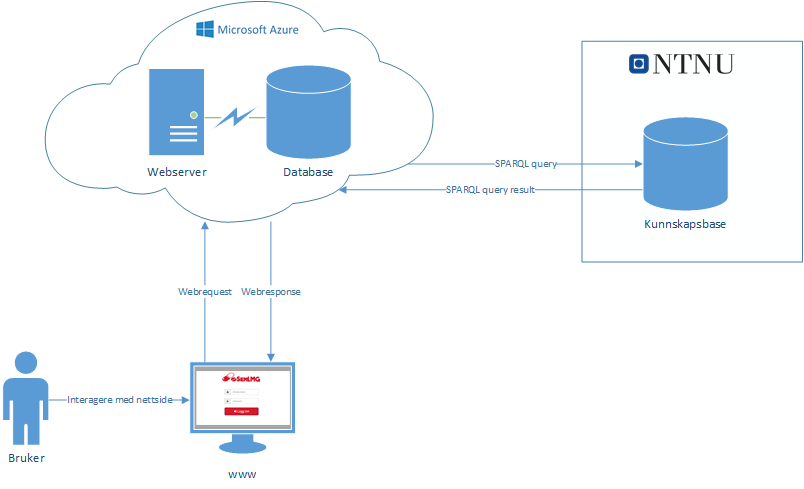
\includegraphics[width=14cm]{images/designview.png}
\caption{Designarkitekturen til SemLMG}
\label{fig:designview}
\end{figure}
Dette er et teknisk oversiktsbilde over hvordan vi ønsket å designe systemet. Brukeren skulle interagere med et webgrensesnitt som kommuniserer med et miljø som eksisterte i Microsoft Azure (skytjeneste). I skyen skulle web-forespørsler håndteres og kontrolleres for å dermed sende web-svar slik at webgrensesnittet ble oppdatert riktig og presentert for brukeren. Når brukeren sendte web-forespørsler hvor skyen trengte å kommunisere med kunnskapsbasen ble det laget \gls{sparql} spørringer til en tjener ved NTNU. Denne tjeneren skulle levere kunnskap om legemiddelgjennomgang og sende dette tilbake som \gls{sparql} resultat som måtte håndteres i skyen og dermed oppdatere webgrensesnittet.
\subsection{Teknologivalg}
I figur \ref{fig:designviewmedteknologi} har vi utvidet designarkitekturen med teknologi og vi ønsker å legge frem for valg av teknologien.
\begin{figure}[H]
\centering
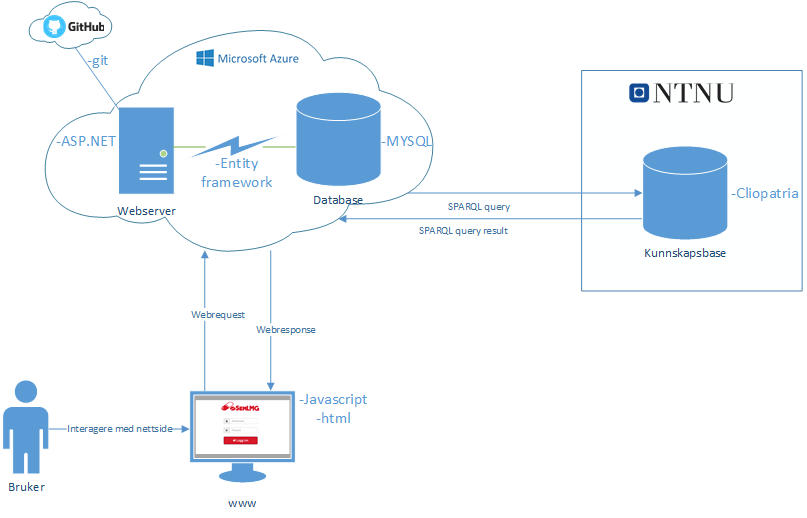
\includegraphics[width=14cm]{images/DesignViewMedTeknologi.png}
\caption{Design perspektivet til SemLMG}
\label{fig:designviewmedteknologi}
\end{figure}
\subsubsection{Webgrensesnitt}

Behovet for å ha et system som kunne være fritt tilgjengelig hvor og når som helst var den høyeste motivasjonen for å utvikle et webgrensesnitt. Etter samtale med biveiledere virket det mest sannsynlig at forsøkspersonene kom til å utføre forsøket på ulike tider i løpet av forsøksuken. Vi ønsket også at det skulle være enkelt for oss å deployere prosjektet. Fordelen var at vi unngikk behovet for å installere noe som helst og at prototypen kunne brukes når og hvor som helst. Grunnet valg av hostingteknologi ble webgrensesnittet bygget opp av Javascript og Html.
\begin{figure}[H]
\centering
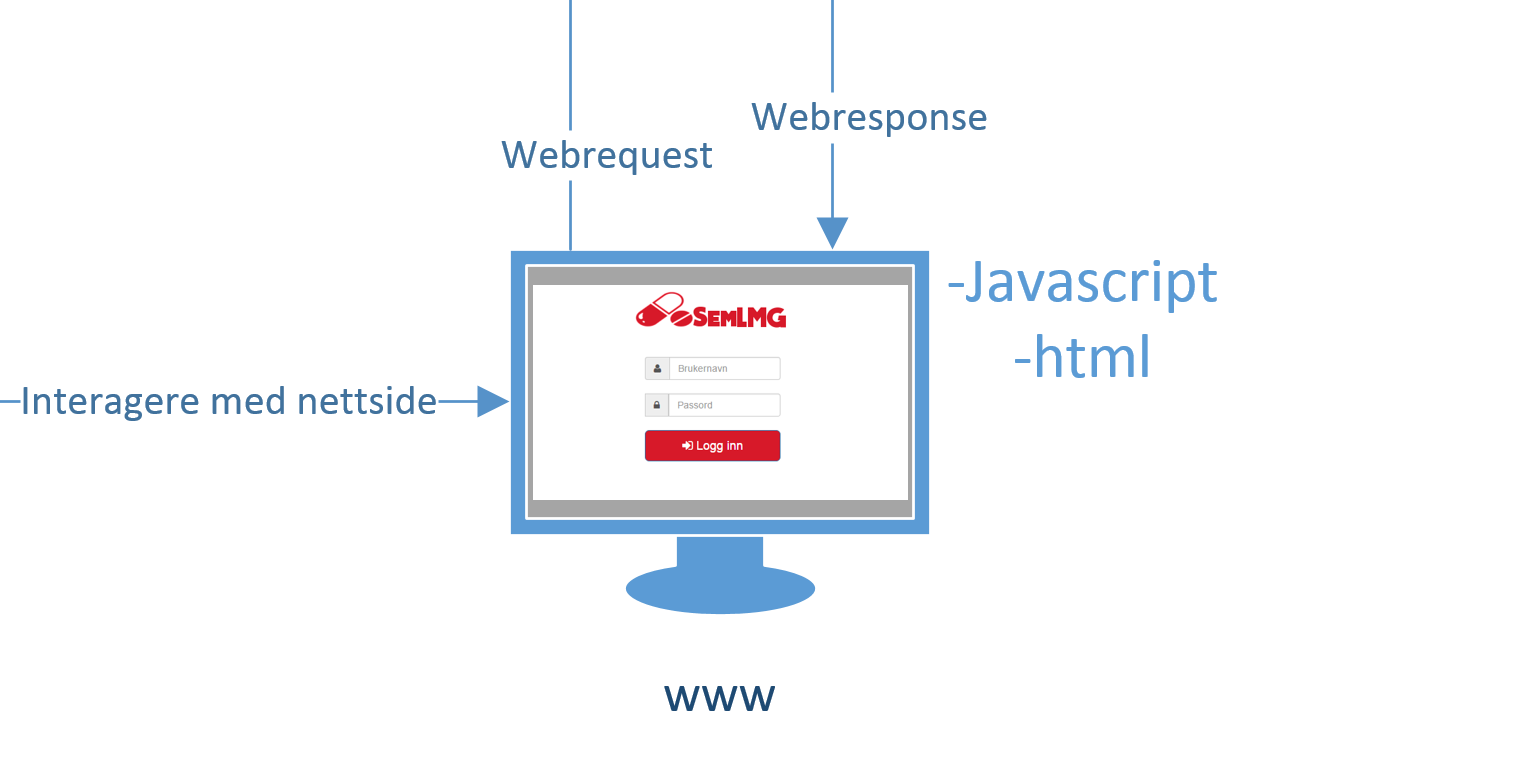
\includegraphics[width=10cm]{images/www}
\caption{Webgrensesnittets teknologi i SemLMG}
\label{fig:webui}
\end{figure}

\subsubsection{Microsoft Azure for hosting}
Oppdagelsen av Azure som hostingpartner kom av at vi lå merke til at studenter ved NTNU har studentlisens på Azure. Vi ble da nysgjerrig på hvordan dette virket og ville prøve oss frem. Azure leverer akkurat det vi trenger for vårt formål og er enkelt å sette opp. I Azure kan vi deployere en eller flere web applikasjoner, opprette database, bruke Azures egne domener og samtidig ha full oversikt over trafikk.
\begin{figure}[H]
\centering
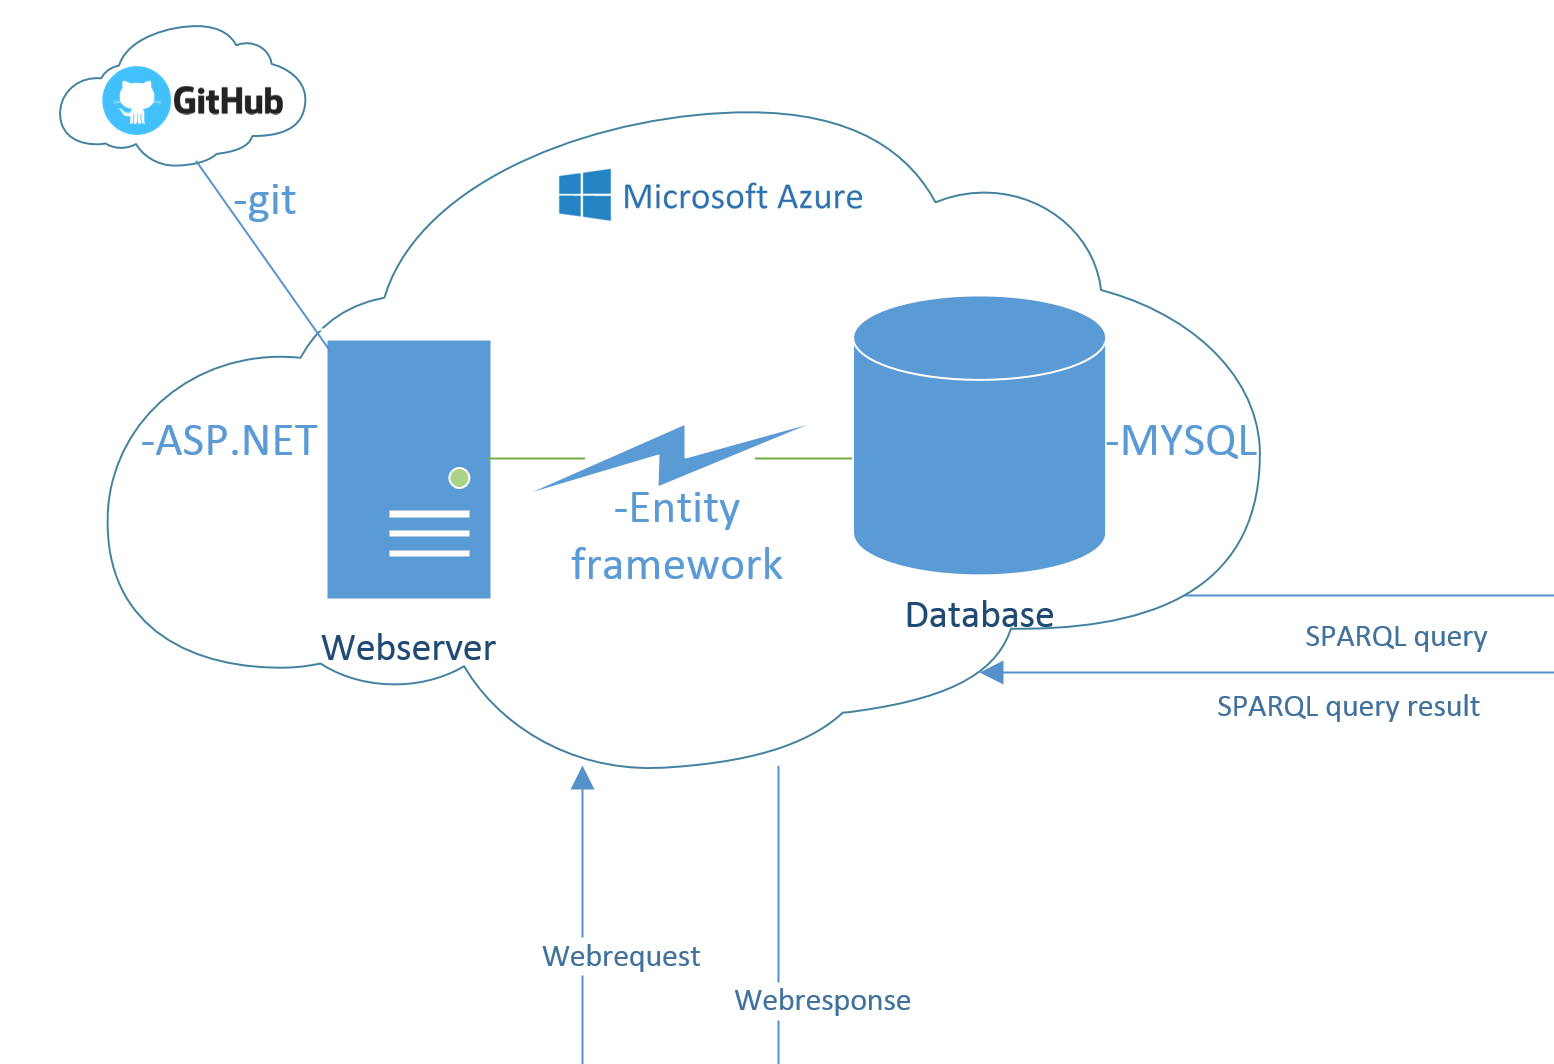
\includegraphics[width=10cm]{images/sky}
\caption{Azure-skytjeneste i SemLMG}
\label{fig:sky}
\end{figure}
\subsubsection{.NET som utviklingsplatform}
Grunnlaget for å utvikle under .NET platformen kom av at alle i mastergruppen hadde erfaring med dette og kommer til å jobbe på samme platform etter masteroppgave. Når det ble avtalt at vi skulle lage et webgrensesnitt tok vi også beslutningen om å utvikle dette under ASP.NET platformen. I ettertid var dette et godt valgt da MedExt-systemet var tilgjengelig i C\#, noe som førte til at integrasjonsprosessen ble enklere.
\subsubsection{Webserver}
Webserveren deployerte som sagt et ASP.NET prosjekt. Dette prosjektet var utviklet ved bruk av MVC-prinsippet (forklart nærmere i MVC-prinsippet i kap. \ref{chap:mvc}) og kommuniserte med en MYSQL database ved bruk av Entity-Framework rammeverket. Webserveren håndterte web-forespørsler ved å sende web-svar for å oppdatere riktig webgrensesnitt. Hvis brukeren sendte web-forespørsler som hadde behov for å  lagre i databasen vil den bruke Entity-Framework til å lagre i riktig tabell. Hvis brukeren sendte web-forespørsler som krevde kompetansen fra kunnskapsbasen ville den spørre kunnskapsbasen og oppdatere grensesnitt med svar fra kunnskapsbasen. Mer om designet til webapplikasjonen i kap \ref{chap:webapp}.
\subsubsection{Database}
For å kunne ha kasuistikker og resultater fra forsøket hadde vi behov for en database å kunne lagre i. Valget falt dermed på å sette opp en MYSQL database i Azure som webserveren har direkte tilgang til. Mer om designet til databasen i kap \ref{chap:db}.
\subsubsection{GIT som versjonskontrollsystem}
Hele mastergruppen har erfaring med Git og det ble derfor naturlig å bruke dette. Som studenter ved NTNU har vi studentlisens på Github som gjør at vi kan holde prosjektet vårt lukket som privat prosjekt. Azure kommuniserer godt med Github, og vi fant etterhvert ut at vi kunne deployere prosjektet vårt kontinuerlig fra Github. For å deployere leser Azure fra en bestemt Branch i et Github repository og deployere hva enn det må være der. Azure har også fine loggmuligheter og vi kan se om vi har noen feil i Branchen vår når den prøver å bygge prosjektet før deployering.

\subsubsection{Kunnskapsbase}
Ved NTNU står det en tjener som fungerer som en grafdatabase (tripplestore).Denne fikk vi erfaring med våren 2015 hvor vi hadde et prosjekt i emnet Web intelligens. Vi ønsket derfor å fortsette å bruke denne tjeneren som et endepunkt for vår kunnskapsbase. Teknologien som ligger i bunn for å kunne få en grafdatabase opp å gå er Cliopatria. Mer om designet til kunnskapsbasen i kap \ref{chap:kunnskapsbasedesign}.
\begin{figure}[H]
\centering
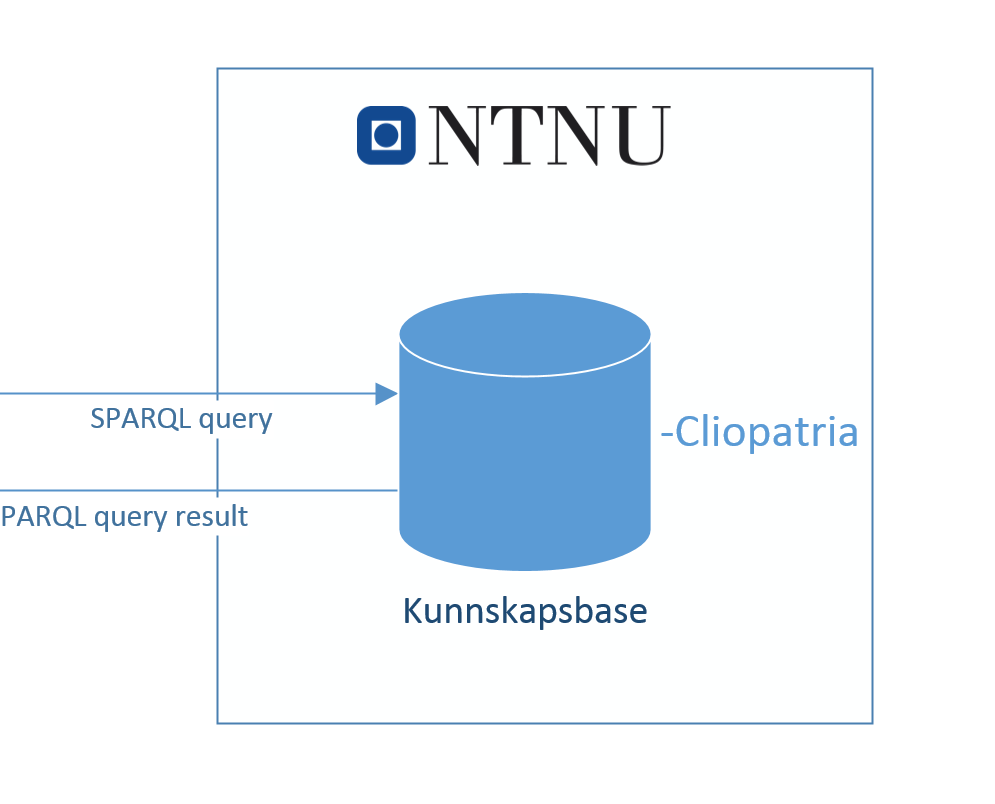
\includegraphics[width=10cm]{images/pille}
\caption{Azure-skytjeneste i SemLMG}
\label{fig:pille}
\end{figure}

\subsection{Webapplikasjonen}
\label{chap:webapp}
\subsubsection{Model-View-Controller arkitektonisk mønster}
\label{chap:mvc}
\gls{mvc} mønsteret er et arkitektonisk mønster brukt i programvareutvikling. Motivasjonen bak ligger i utvikling av grensesnitt. \gls{mvc} var en av de første tilnærmingene for å beskrive og implementere programvarekunstruksjoner i form av ansvarsområdet. \gls{mvc} mønsteret ble formulert av Trygve Reenskaug i 1970 og senere uttrykt som et generelt konsept i 1988 i en artikkel i The Journal of Object Techonology. \\
Målet med \gls{mvc} er å kunne skille på ansvaret til de ulike delene av systemet. For vedlikehold trenger ikke de ytre delene av systemet å vite noe om hvordan de indre delene ser ut, men heller andre veien. Kontrollerklasser vet alt om modellklasene, men ikke vice versa. Første tilknytningspunkt til brukeren vil være kontrolleren. Ansvaret til en kontrollerklasse vil være å sende meldinger til modellen om å oppdatere data. Dermed vil den sende meldinger til viewet om å oppdatere grensesnittet med riktig data. Modelklasser vil ha ansvaret for å modellere data og ha koblinger mot en database. Viewklasser har ansvar for de forskjellige grensesnittene og har ansvar for å oppdatere grensesnittene med riktig data.
Noe mer vanlig er å bruke en annen implementasjon av Model-view-conroller for å kunne binde flere modeller sammen og bruke i et view. Denne implementasjonen heter \gls{mvvm} og introduserer en ekstra ansvarsdel som heter viewmodel, som vist i figur \ref{fig:mvvm}. Dette er noe som ble brukt i utviklingen av webapplikasjonen da vi for eksempel hadde behov for å binde både en bruker med en kasuistikk og presentere data fra begge modellene. Her vil modellen endre seg med at viewmodelklassene vil binde sammen data fra modellene og grensesnittet for å kunne preseneteres for brukeren.
\begin{figure}[H]
\centering
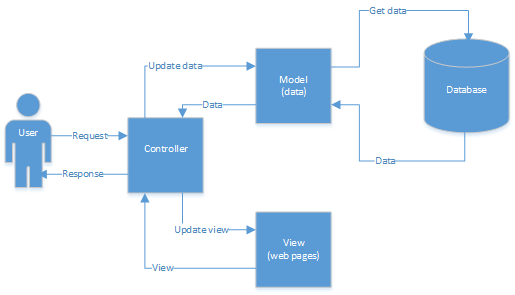
\includegraphics[width=14cm]{images/mvc}
\caption{MVC-mønsteret brukt i SemLMG}
\label{fig:mvc}
\end{figure}

\begin{figure}[H]
\centering
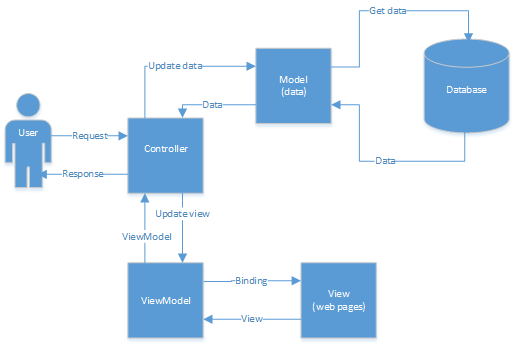
\includegraphics[width=14cm]{images/mvvm}
\caption{MVVM-mønsteret brukt i SemLMG}
\label{fig:mvvm}
\end{figure}

\newpage
\subsubsection{Entity framework}
For å enkelt kunne opprette, slette og endre databasen har vi valgt å bruke en objekt-relasjonsmapper kalt Entity framework. Dette eliminerer behovet for å skrive data-aksess kode mellom modellen og databasen. Entity framework viste seg å være et ganske kraftig verktøy for å opprette tabeller og databaser i det hele tatt. Etter å ha utforsket miljøet litt fant vi ut at vi kunne opprette hele databasebehovet vårt ved hjelp av code-first prinsipper med Entity framework. Code-first prinsippet går ut på at du ved annotasjoner i klassene dine bestemmer hva som er tabeller og hvilke datatyper som skal være attributter i tabellen i databasen. Når vi har satt opp alle klasser med datatyper er det bare å kjøre en migrasjon mot databasen og oppdatere den. Et slikt prinsipp viste seg å være kraftig når det gjelder konsistens. Hvis tabellene allerede finnes og modellene har endret seg, vil entity framework be deg om å kjøre en ny migrering slik at både kode og database har like forhold. Har du valgt code-first prinsipp så vil databasen da følge koden og ikke andre veien.
\begin{figure}[H]
\centering
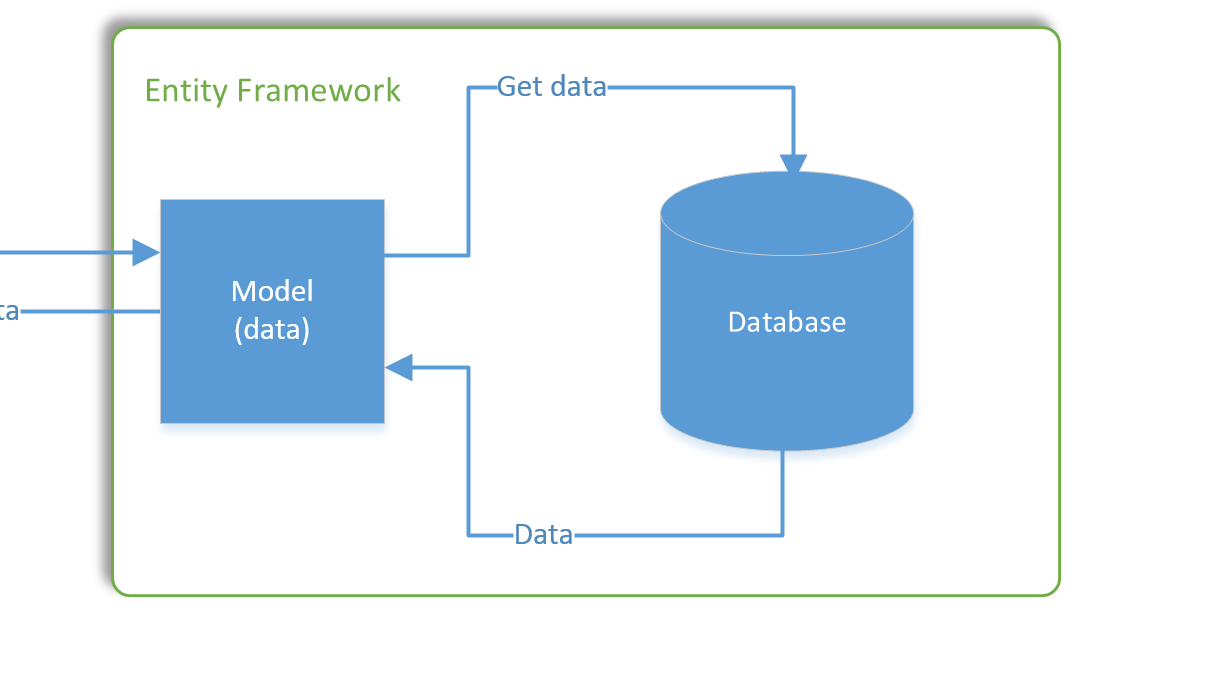
\includegraphics[width=14cm]{images/EntityFramework}
\caption{Entity framework kobling}
\label{fig:entityframework}
\end{figure}
\subsubsection{Samstemmingsverktøy}
Vår webapplikasjon gjenbrukte det nåværende samstemmingsverktøyet MedExt for å kunne trekke ut legemiddelinformasjon fra friteksten i kasuistikkene. Når brukeren var logget inn og ser kasuistikken må brukeren trykke ''Neste''-knappen for å gå videre i eksperimentet. Når denne klikkes gikk man videre og fikk se en liste over legemidler. Mellom disse vinduene var samstemmingsmodulen brukt. Samstemmingsmodulen tar inn fritekst, og gir ut en tekststreng i xml-format. Hvert enkelt legemiddel i denne tekststrenger blir da serialisert til legemiddelobjekter med tilhørende attributter som dose, doseringsenhet, frekvens og ATC-kode. 

\subsubsection{Design-klassemodellen}
For å få en forståelse for hvordan webapplikasjonen var bygd opp har vi modellert et klassediagram. Denne er representert i \ref{fig:classDiagram}. I modellen ser vi spor av MVVM-prinsippet. Vi har to base-klasser for kontroller- og viewmodel klasser. Model-klassene finner vi øver til høyre hvor vi finner Case,MedicalReview,CaseResult og User. Context-klassene er koblinger til database og fungrer som et knutepunkt mellom kontrollerne og modellene.
\begin{figure}[H]
\centering
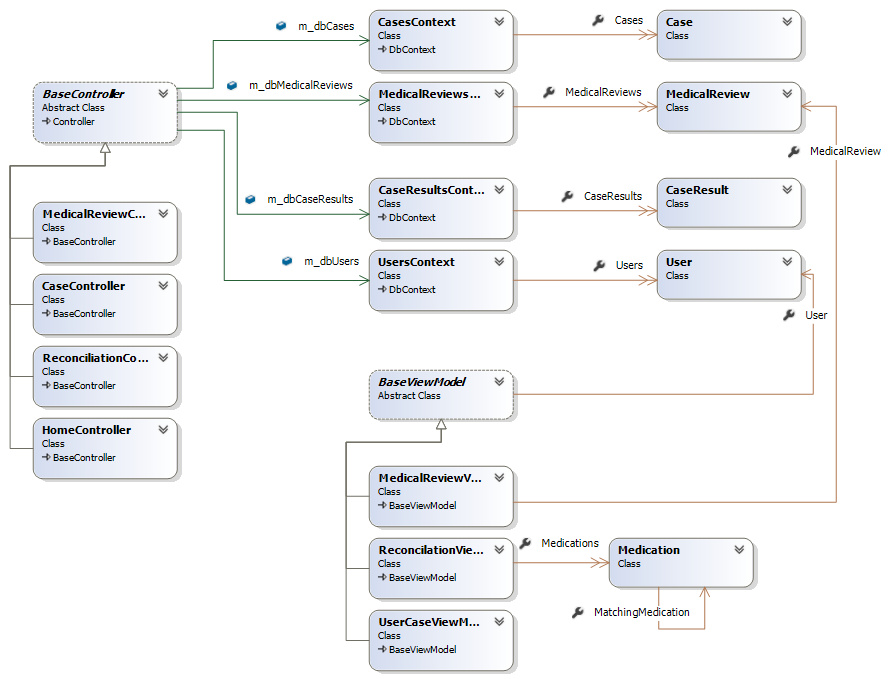
\includegraphics[width=14cm]{images/ClassDiagram.png}
\caption{Klassediagram for webgrensesnitt}
\label{fig:classDiagram}
\end{figure}

Vi ønsker å beskrive klassene dypere. Under vil vi ta for oss klassene som følger MVVM-prinsippet. Vi ønsker ikke å gå dypere inn i Context-klassene, da disse arver fra Entity Framework og krever bare at du spesifiserer hvilke modell-klasser som skal speiles med database. \\

\textbf{BaseController-klassehiarkiet} \\
I ASP.NET prosjekter blir klasser som har kontrollen på grensesnittet ofte referert til som kontroller-klasser. I figur \ref{fig:basecontroller} ser vi at vi hadde laget et grensesnitt med 4 forskjellige views. Dette var da de 4 sidene som skulle vises i webgrensesnittet. Hver av disse klassene arvet metoder fra BaseController for å kunne ha en felles måte å styre brukeren frem og tilbake mellom de forskjellige sidene. BaseController hadde også objekter for Context-klassene. Disse ble arvet på samme måte og betyr at på en hver side kunne vi gjøre endringer i databasen ved behov.
\begin{figure}[H]
\centering
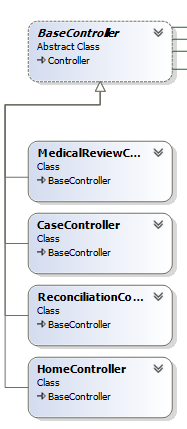
\includegraphics[width=4cm]{images/BaseController.png}
\caption{BaseController-klassehiarkiet}
\label{fig:basecontroller}
\end{figure}


\textbf{BaseViewModel-klassehiarkiet} 

Viewmodeller i vår webapplikasjon var designet til å kunne binde flere modeller sammen. Hos oss var vi alltid avhengig av at de forskjellige sidene hadde tilgang til en bruker samt en kasuistikk. Vi ser i figur \ref{fig:baseviewmodel} at navnene skal representere hva de inneholder. F.eks \textit{UserCaseViewModel} vil inneholde en binding mellom User og Case-klassene . 

Klassene var designet etter hvor de skal brukes. I vår webapplikasjon hadde vi en variabel som holdt styr på brukeren. Dette var en variabel som skal brukes på alle sider, og var dermed plassert i \textit{BaseViewModel} slik at alle viewmodellene kunne arve og bruke den. Det fantes naturligvis tilstander og hendelser som bare skulle skje på spesifikke sider, og disse var da plassert i de tilhørende viewmodellene. F.eks \textit{MedicalReviewViewModel} skulle ha holde styr på hvilke forsøkspersoner som skulle se forslag til tiltak eller ikke. Denne hadde da en boolsk variabel som ville endre seg etter hvilken bruker som var logget inn. Grensesnittet leste denne og endrer grensesnittet basert på verdien.
\begin{figure}[H]
\centering
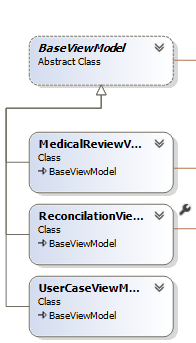
\includegraphics[width=4cm]{images/BaseViewModel.png}
\caption{BaseViewModel-klassehiarkiet}
\label{fig:baseviewmodel}
\end{figure}


\newpage
\textbf{Medication}

Når en samstemming ble gjort fikk vi legemidlene i et XML-format. Vi trengte \textit{Medication} klassen for å kunne hente ut attributter og sette de inn i et logisk objekt som vi kunne bruke senere. Medication klassen har dermed attributtene \textit{MedicationName},\textit{AtcCode},\textit{DosageValue},\textit{DosageUnit},\textit{Frequency}. Denne ble også brukt mot kunnskapsbasen for å kunne hente ut tiltak for hvert legemiddel.
\begin{figure}[H]
\centering
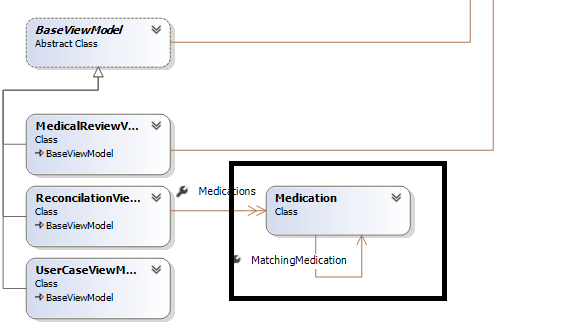
\includegraphics[width=10cm]{images/Medication.png}
\caption{Medication-klasse}
\label{fig:Medication}
\end{figure}


\textbf{Modell-klasser} 

Modell-klassene var basisen for hele prosjektet. Her har vi klassene \textit{User},\textit{Case},\textit{MedicalReview},\textit{CaseResult}. \textit{User} inneholder informasjon om en bruker som logger seg inn og gjennomfører eksperimentet.En hver \textit{User} er koblet sammen med en \textit{Case}, men denne koblingen ligger i \textit{Context-klassene}. \textit{Case} inneholder kasuistikk-teksten og er koblet sammen med \textit{CaseResult}. \textit{CaseResult} inneholder måling av tid på de forskjellige sidene i grensesnittet, dette er for å måle tiden det tar for brukere og utføre de forskjellige delene av eksperimentet. \textit{CaseResult} er koblet sammen med \textit{MedicalReview}. \textit{MedicalReview} inneholder alle tiltakene som blir skrevet inn av brukeren. \\
\begin{figure}[H]
\centering
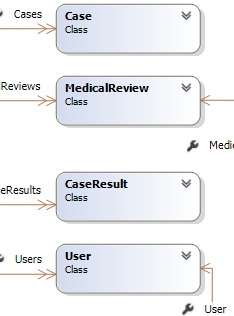
\includegraphics[width=4cm]{images/Models.png}
\caption{Modell-klasser}
\label{fig:models}
\end{figure}
Ved å lage webapplikasjonen på denne måten kunne vi enkelt styre grensesnittet, endre modeller og lagre ønsket informasjon. Vi kunne sjekke opp resultatet på en bruke etter den hadde utført eksperimentet og \textit{Context}-klassene hjalp oss med å lagre i databasen. Dette var hvor vi kunne se resultatene og hente dem ut for å videre analysere dem.


\subsection{Databasemodellen}
For å kunne ha en strukturert samling av relevant data, knyttet vi webapplikasjonen til en MySQL database. Denne databasen hadde som oppgave å bevare data om en bruker og brukerens kasuistikk samt resultater som ble lagret når webappliaksjonen ble brukt. Databasen var en relasjonsdatabase og følger de mest vanligste prinsippene for å kunne oppnå relasjoner mellom data. \\

I figur \ref{fig:umldiagramdatabase} er det modellert en UML representasjon av databasen. Videre ønsker vi å forklare nærmere hva hver tabell brukes til og trekke ut de viktigste attributtene i tabellen. *-symbolet etter et attributt betyr at dette attributtet er en primærnøkkel\footnote{En primærnøkkel er en unik verdi som vil identifisere en rad i tabellen} i tabellen. \underline{Understreket} attributt betyr at attributtet er en fremmednøkkel\footnote{ En fremmednøkkel er en referanseverdi til en rad i en annen tabell, dette er den mest vanligste metoden for å kunne ha relasjonsmønstre i en database} i tabellen.
%\end{description}
\begin{figure}[H]
\centering
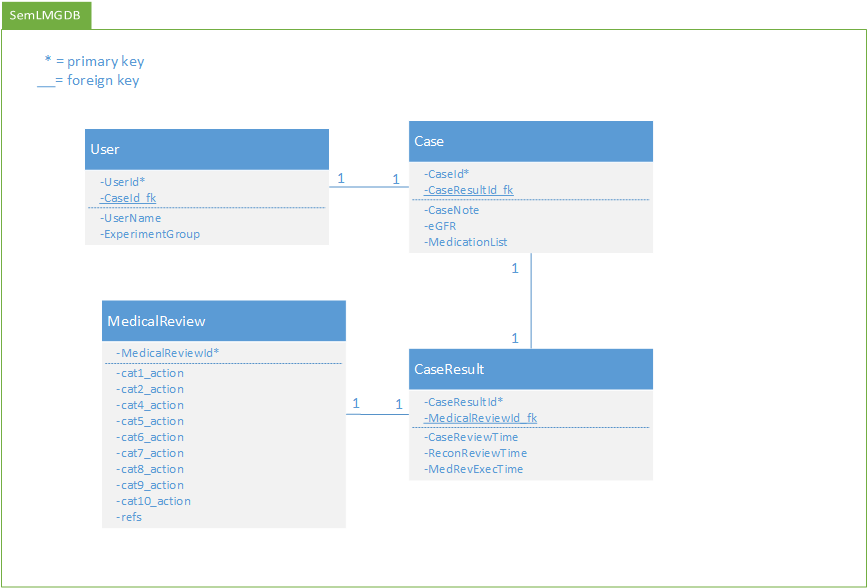
\includegraphics[width=16cm]{images/UMLDiagramDatabase.png}
\caption{UML diagram av database}
\label{fig:umldiagramdatabase}
\end{figure}
\label{chap:db}

\begin{description}
\newpage

\item[User]
var en tabell som skulle inneholde informasjon om en bruker.
\begin{description}
\item[UserName] var en streng som inneholdt brukernavnet til brukeren ved innlogging.
\item[ExperimentGroup] var et heltall som ville variere mellom 1 og 2. Verdien brukes til å skille mellom hvilke brukere som skulle få presentert en tiltaksliste eller ikke.
\end{description}

\item[Case] var en tabell skulle inneholde informasjon om en kasustikk. 
\begin{description}
\item[CaseNote] var en streng som ville inneholde hele teksten fra kasuistikken. Denne ville også være formatert i html-kodeformat for å kunne bli presentert i webgrensesnittet.
\item[eGFR] var et heltall som skulle bevare eGFR-verdien til kasuistikken. Denne ble brukt til å gjøre spørringer mot kunnskapsbasen.
\item[MedicationList] var en streng som inneholdt alle medisinene som ble nevnt i kasuistikken. Denne listen ble tolket av MedEXT og ble brukt til å gjøre spørringer mot kunnskapsbasen.
\end{description}

\item[CaseResult] var en tabell som skulle inneholde tidsmålinger på brukeren når brukeren navigerte seg frem og tilbake i applikasjonen. Webapplikasjonen hadde tre skjermbilder som det var interessant å måle tid på. Disse tre vinduene er lagrer tid en bruker i hvert vindu i tilsvarende \textbf{CaseReviewTime}, \textbf{ReconReviewTime} og \textbf{MedRevExecTime}.

\item[MedicalReview]  var en tabell som skulle inneholde informasjon om tiltakene som ble tatt og hvor brukeren klikker under LMG.
\begin{description}
\item[catX\_action] var en attributt som ble brukt for lagring av tiltak for kategorier. Disse tiltakene var det bruker som førte inn. Vi hadde 10 kategorier i LMG-skjemaet og dermed 10 attributter for hver kategori i databasen.
\item[refs] var en attributt som skulle lagre om en bruker hadde klikket på ''Bruk tiltak'' eller ''Les kilde''. Dette er en streng som blir tilføyd etterhvert som brukeren klikker på disse to knappene i grensesnittet.
\end{description}

\end{description}



\subsection{Kunnskapsbase}
\label{chap:kunnskapsbasedesign}
I kunnskapsbasen lå ontologien lagret. Til lagring av ontologien brukte vi Cliopatria, er en web server med et enkelt grensesnitt for å laste opp RDF filer.  Ontologien ble bygget ved bruk av verktøyet Protégé og lastet opp i Cliopatria, et triplestore basert på prolog. Protégé tilbyr et enkelt grensesnitt for å designe ontologien og populere den med individer(data). Cliopatria ga oss et web grensesnitt og et \gls{sparql} endpoint. Dette SPARQL-endpointet er det vi brukte for å sende spørringer fra prototypen ned til triplestoret. Spørringene har likheter med SQL, vi ''joiner'' data fra ulike deler av RDF-grafen.

Ontologien til prototypen er modellert i Figur \ref{fig:ont}. Modellen består av firkanter som representerer objekter, sirkler som representerer literaler og piler som representerer predikater. 

Under skal vi beskrive strukturen på ontologien i Figur \ref{fig:ont}:
\begin{description}

\item[Drug]
Et legemiddel, beskrevet med handelsnavnet. For eksempel Paracet som er handelsnavnet til medikamentet. I Paracet er det Paracetamol som er det aktive virkestoffet.

Predikater forbunnet med et Drug:
\begin{description}
\item[HasSubstance]
Et drug har predikat som binder det til et eller flere virkestoff. 
\end{description}


\item[Substance]
Substance er virkestoffet til legemiddelet. Det er virkestoffet som er den aktive ingrediensen i legemiddelet.

Predikater forbunnet med et Substance:
\begin{description}
\item[HasRecommandation]
Et Substance har predikat som binder det til et eller flere Recommandations. 
\end{description}


\item[Recommandation]
En Recommandation er anbefalingene til et virkestoff. Et virkestoff har ofte flere anbefalinger og i denne oppgaven har vi tatt hensyn til de anbefalingene som blir gitt ved nedsatt nyrefunksjon. 

Predikater forbunnet med en Recommandation:
\begin{description}
\item[LowerGFR og UpperGFR]
LowerGFR og UpperGFR er grensene for en Recommandation. En Recommandation er gyldig i et visst intervall  for eksempel ''GFR \textgreater 30 og GFR \textless 45''
\item[RecValue]
RecValue er verdien til en Recommandation. Den tekstlige anbefalingen hentet fra \url{www.uptodate.com}.
\item[RecType]
Vi skiller en Recommandation i to forskjellige kategorier ''Doseendring'' og ''Seponering''.
\item[HasSource]
Det er viktig at en Recommandation har en kilde. En Recommandation er koblet mot et Source-objekt ved hjelp av predikatet ''HasSource'' og Source er beskrevet under.
\item[RecID]
RecID er en unik id for anbefalingen. Brukes til å logge hvilke anbefalinger brukeren har brukt.
\item[StrengthOfRecommandation]
StrengthOfRecommandation brukes til å sortere listen over forslag som blir presentert for bruker. Vi sikrer at brukerene får den samme listen og at den blir lik hver gang. Dette parameteret kan brukes til å rangere hvor kritisk en anbefaling er slik at de viktigste anbefalingene kommer øverst.

\end{description}

\item[Source]
Source beskriver kilden til en Recommandation. Kilden er i denne oppgaven en URL til det aktuelle virkestoffet i \url{www.uptodate.com} og innholdet i hele anbefalingen hentet fra overskriften \textbf{Renal Impairment} kilden til en Recommandation. 
\begin{description}
\item[SourceURL]
URL direkte til der RecValue er hentet fra.
\item[SourceText]
Inneholder hele teksten der anbefalingene er hentet fra.
\end{description}
\end{description}

\begin{figure}[H]
\begin{center}
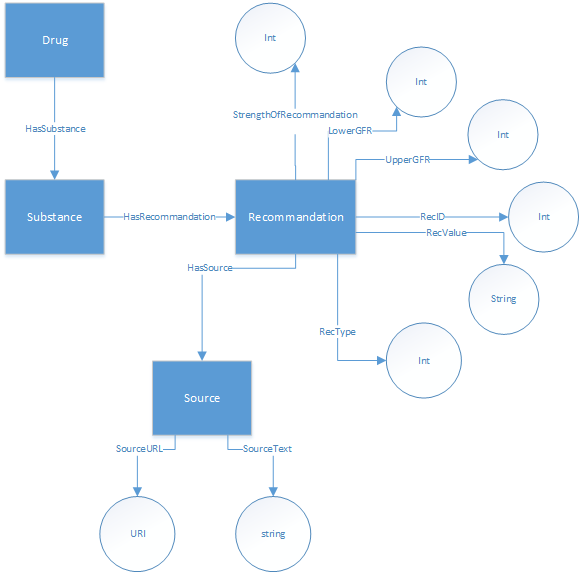
\includegraphics[width=12cm]{images/OntologiDiagram}
\caption{Ontologi modell}
\label{fig:ont}
\end{center}
\end{figure}

\subsection{Grensesnittet mot kunnskapsbasen}
Applikasjonen brukte \gls{sparql} endepunktet som Cliopatria eksponerte på web for å hente data fra ontologien. I \ref{lst:sparql} kan vi se hvordan spørringen er bygget opp og forklart under: 
\begin{description}
    \item[Linje  5 og 6] Her står de verdiene som ble hentet ut. Alle parameterene vi trengte til prototypen. Virkestoff label, recommandation verdi, strengthOfRecommandation, sourceURL, sourceText, recommandation type og Id, alle disse beskrevet i kapittel \ref{chap:kunnskapsbasedesign}.
    \item[Linje 7-17] Input fra systemet er markert i \{0\}, det er enten handelsnavnet til et medikament eller virkestoffet. Vi ser union av to sub-spørringer. Den første brukes hvis det er handelsnavnet av legemiddelet som sendes inn for å finne hvilket virkestoff som er knyttet til et legemiddel. Den andre sub-spørringen henter ut virkestoffet med samme navn som input.
    \item[Linje 19-24] Et virkestoff er knyttet til 0 - flere flere anbefalinger. Anbefalingene er er kun effektive i et intervall mellom to verdier av eGFR. Disse verdiene blir hentet ut fra anbefalingen og så filtrert ut slik at det er kun korrekt anbefaling som blir med lenger ned i spørringen.
    \item[Linje 26-33] Her hentet vi ut all data fra de forskjellige objektene. Navnet fra en ''substance'', forskjellige verdier fra en ''recommandation'' og URL/text fra kilden.
\end{description} 


\section{Demonstrasjon av prototype}
\ot{Husk å oppdatere bilder med nyeste versjon, se over teksten til hvert vindu slik at det passer}
\subsection{Innloggingsvindu}
Figur \ref{fig:demo1} viser forsiden til webapplikasjonen. Her kunne brukere logge inn med tilhørende brukernavn.
\begin{figure}[H]
\begin{center}
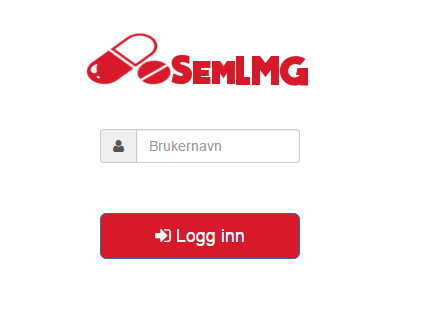
\includegraphics[width=8cm]{images/demoimages/1}
\caption{Innloggingsvindu}
\label{fig:demo1}
\end{center}
\end{figure}
Logoen øverst på siden ble fjernet når eksperimentet ble startet. Dette var for å ikke forvirre/forstyrre deltakeren med en logo som ikke har en funksjon.

\subsection{Kasuistikkvindu}
Figur \ref{fig:demo2} viser kasuistikkvinduet. Etter innlogging ble brukeren presentert for en pasientkasuistikk. Denne kasuistikken skulle brukeren lese og bli kjent med. Når brukeren var ferdig med å lese kasuistikken kunne han trykke ''Neste''.
\begin{figure}[H]
\begin{center}
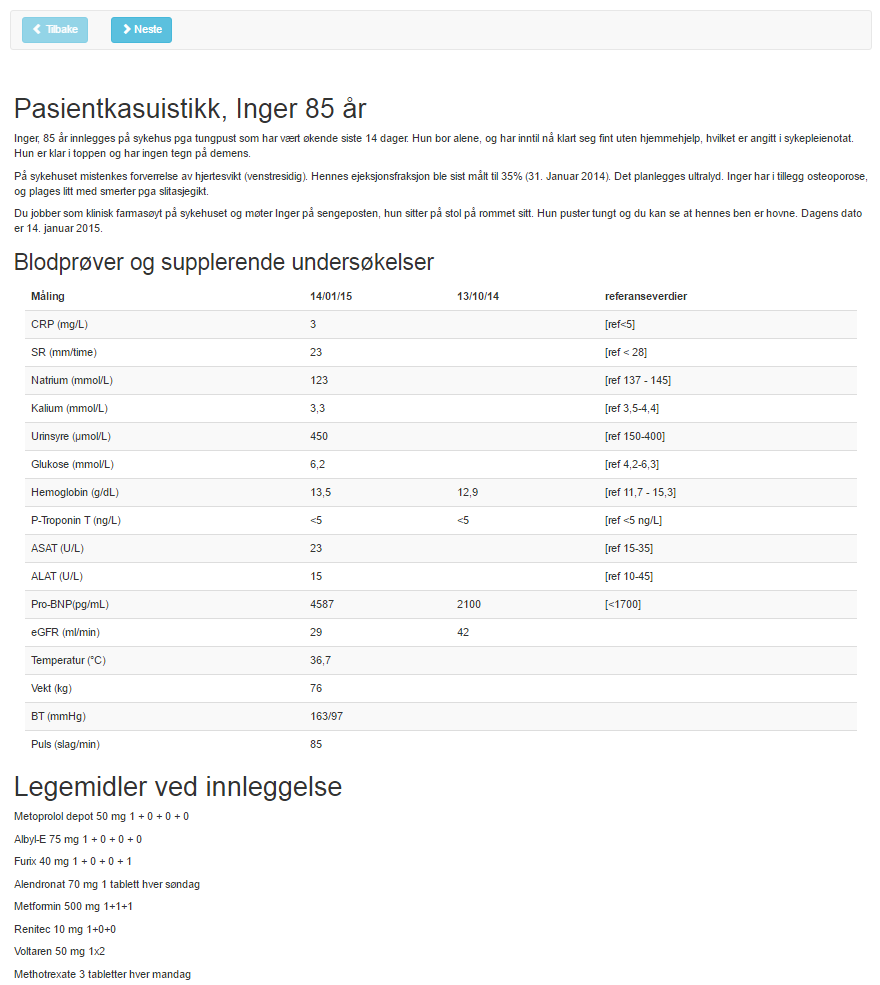
\includegraphics[width=14cm]{images/demoimages/2}
\caption{Kasuistikkvindu}
\label{fig:demo2}
\end{center}
\end{figure}

\newpage
\subsection{Vindu for legemidler i bruk}
Figur \ref{fig:demo3} viser legemidler i bruk vinduet. Dette var et vindu hvor brukeren skulle observere at en LiB-liste ble laget fra pasientkasuistikken. Når brukeren var ferdig med å observere listen kunne de trykke ''Neste''.
\begin{figure}[H]
\begin{center}
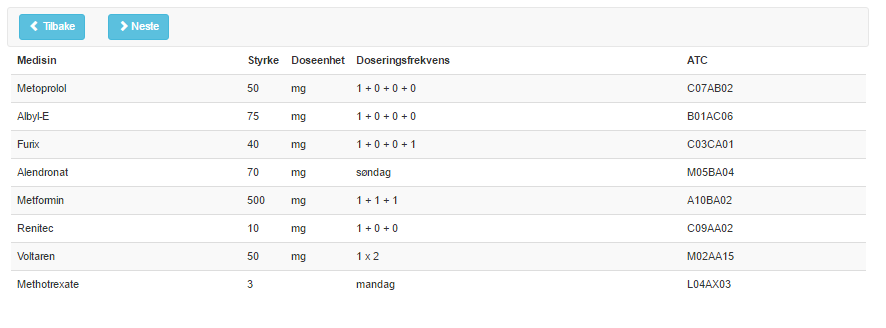
\includegraphics[width=18cm]{images/demoimages/3}
\caption{LiB-vindu}
\label{fig:demo3}
\end{center}
\end{figure}

\newpage
\subsection{Legemiddelgjennomgangvindu}
Figur \ref{fig:demo4} viser legemiddelgjennomgangen som brukeren skulle utføre. Vinduet bestod av et lignende skjema som kliniske farmasøyter bruker i dag. Dette er et skjema som blir fylt ut når farmasøyter finner forslag til tiltak under en legemiddelgjennomgang. I figur \ref{fig:demo4} hadde brukeren muligheten til å se forslag til tiltak under en bestemt kategori. Dette er kategorien som vil inneholde tiltak for nedsatt nyre og leverfunksjon. Vinduet består også av den samstemte legemiddellisten (til høyre) og kasuistikken (nederst).
\begin{figure}[H]
\begin{center}
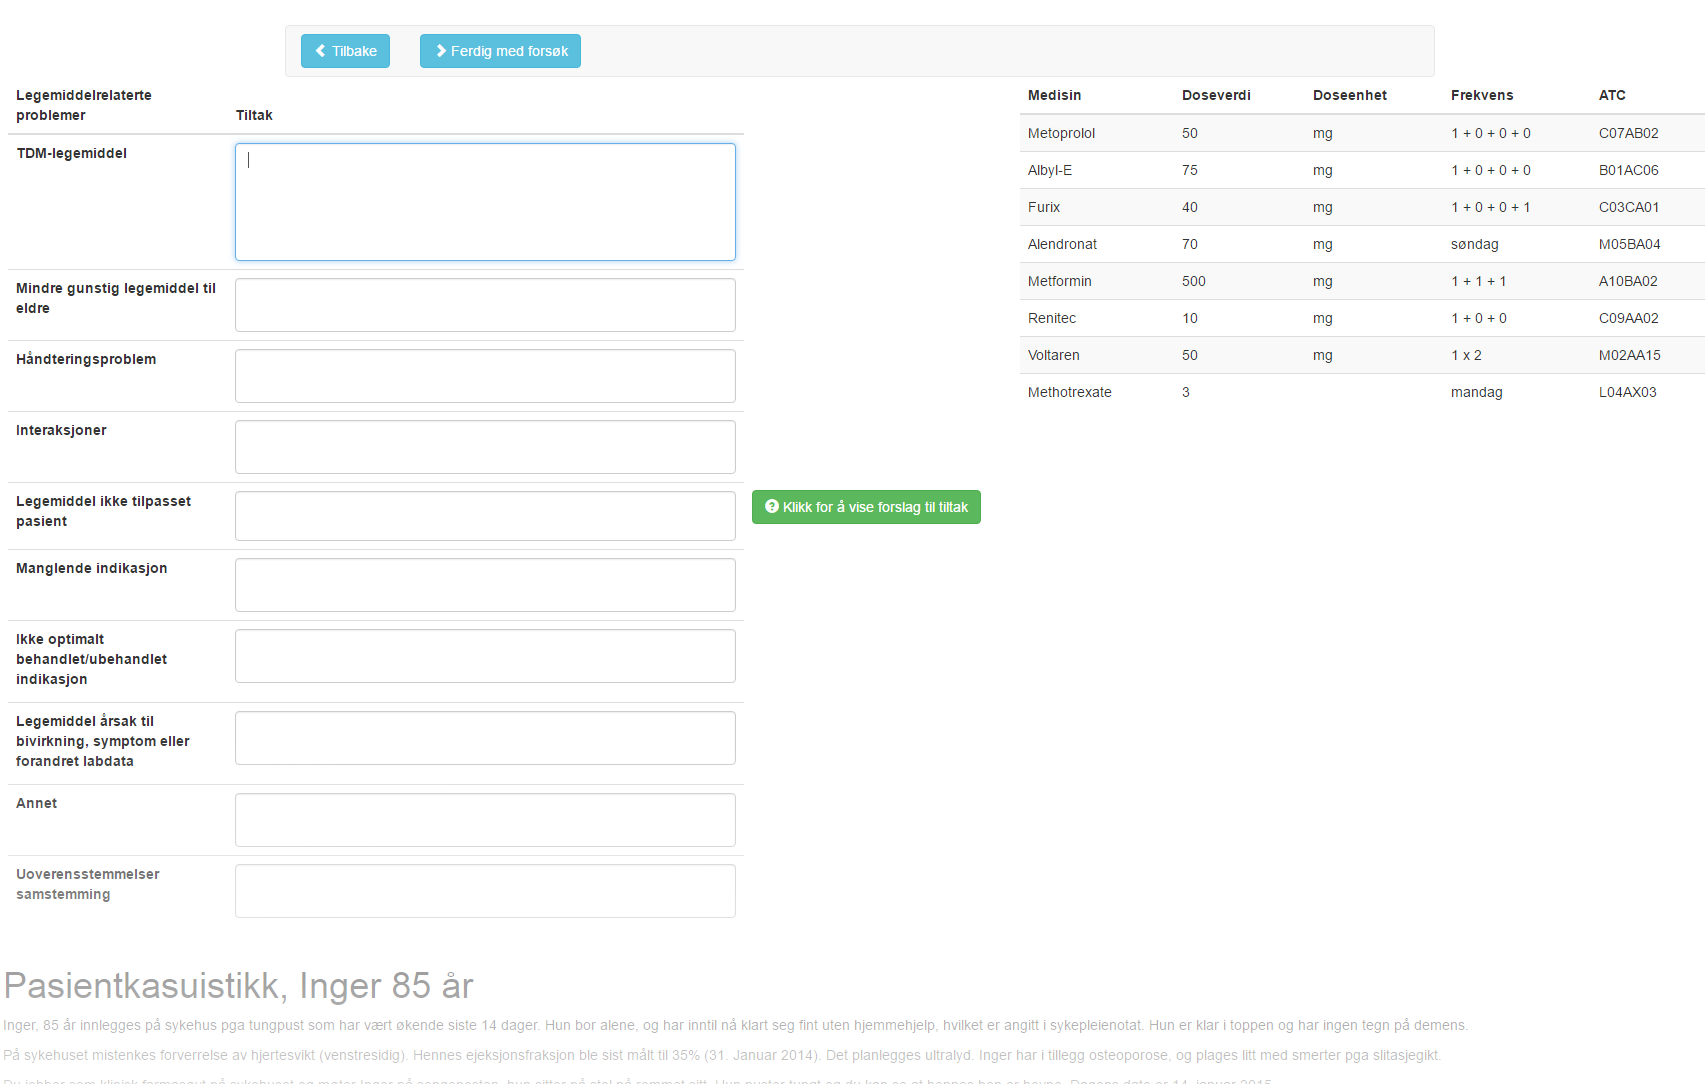
\includegraphics[width=18cm]{images/demoimages/4}
\caption{LMG-vindu}
\label{fig:demo4}
\end{center}
\end{figure}
\newpage
 Hvis brukeren trykte på knappen ''Klikk for å vise forslag til tiltak'' ville en liste med forslag dukke opp under legemiddellisten (høyre). I figur \ref{fig:demo5} ser vi at grensesnittet har forandret seg til hvordan det så ut når en bruker ønsket å se listen.
\begin{figure}[H]
\begin{center}
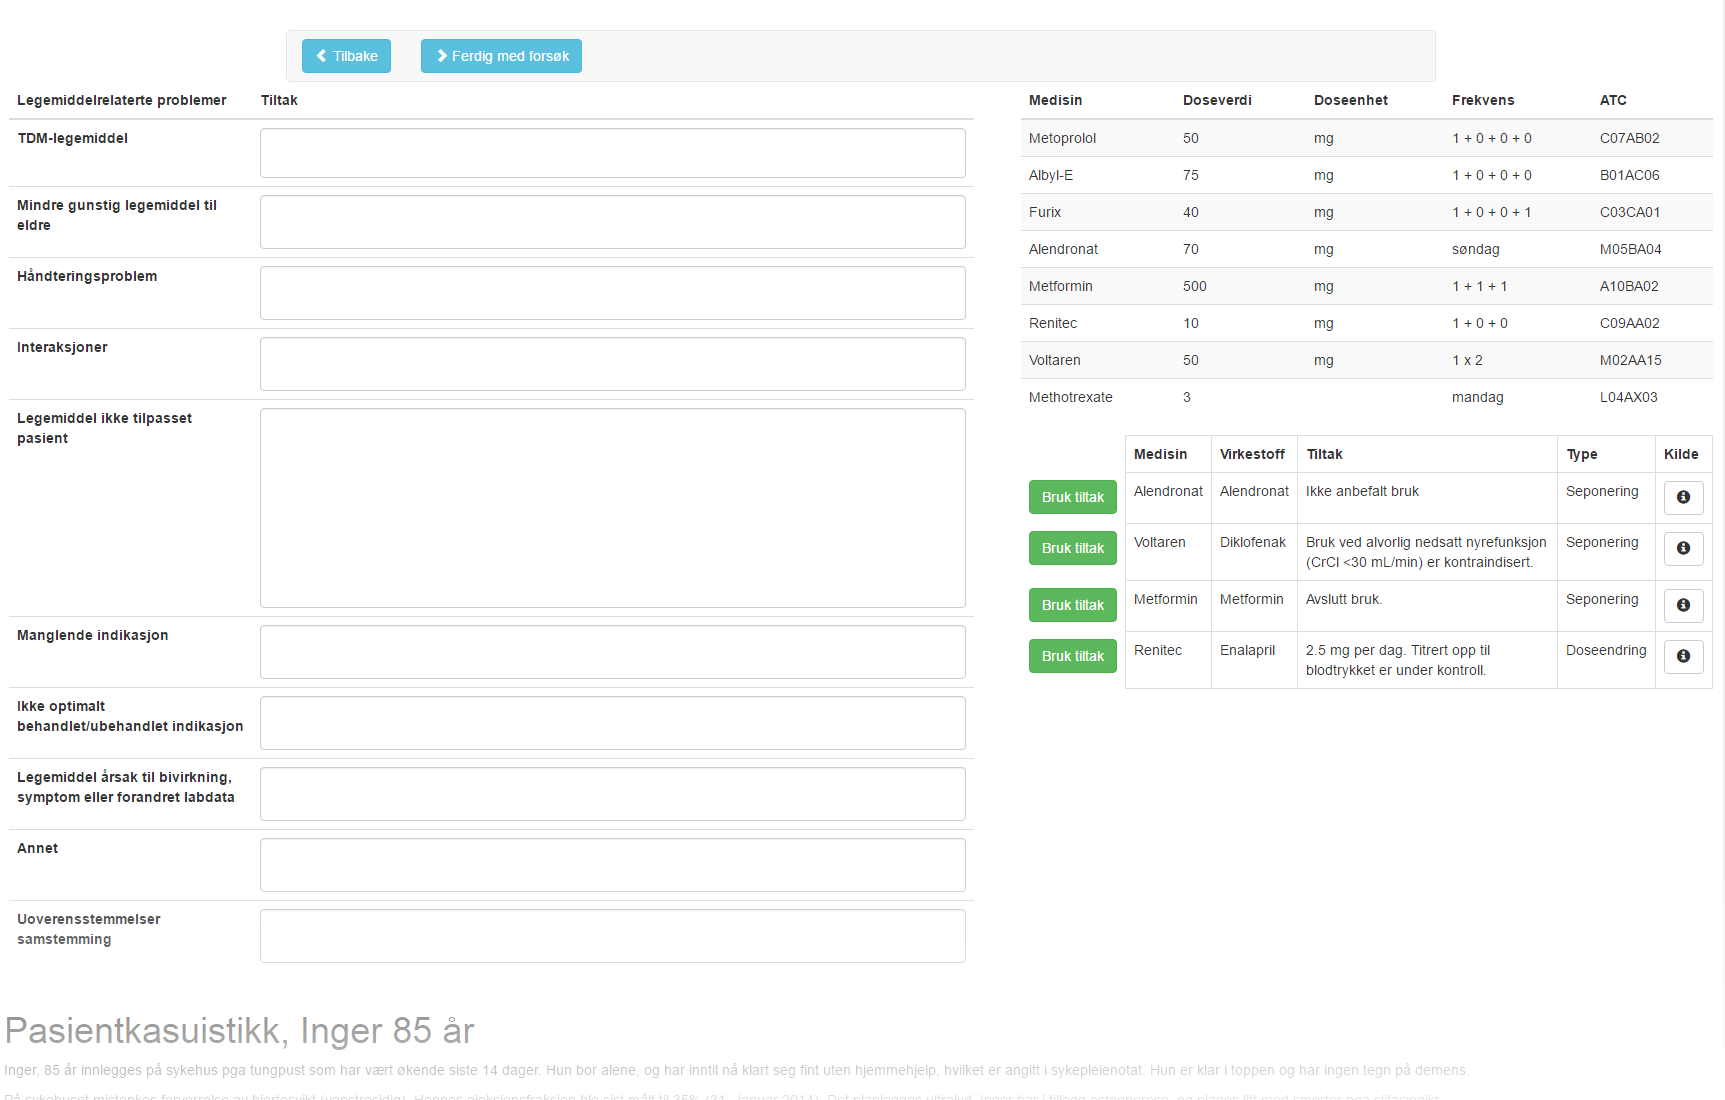
\includegraphics[width=18cm]{images/demoimages/5}
\caption{LMG-vindu med forslag til tiltak}
\label{fig:demo5}
\end{center}
\end{figure}
\newpage
 I denne listen kunne brukeren velge å bruke tiltak. Disse tiltakene ble da automatisk skrevet inn i tiltaksfeltet i skjemaet. Dette kan vi se i figur \ref{fig:demo6}. Når brukeren følte seg ferdig med LMG-skjemaet kunne man presse ''Ferdig med forsøk''.
\begin{figure}[H]
\begin{center}
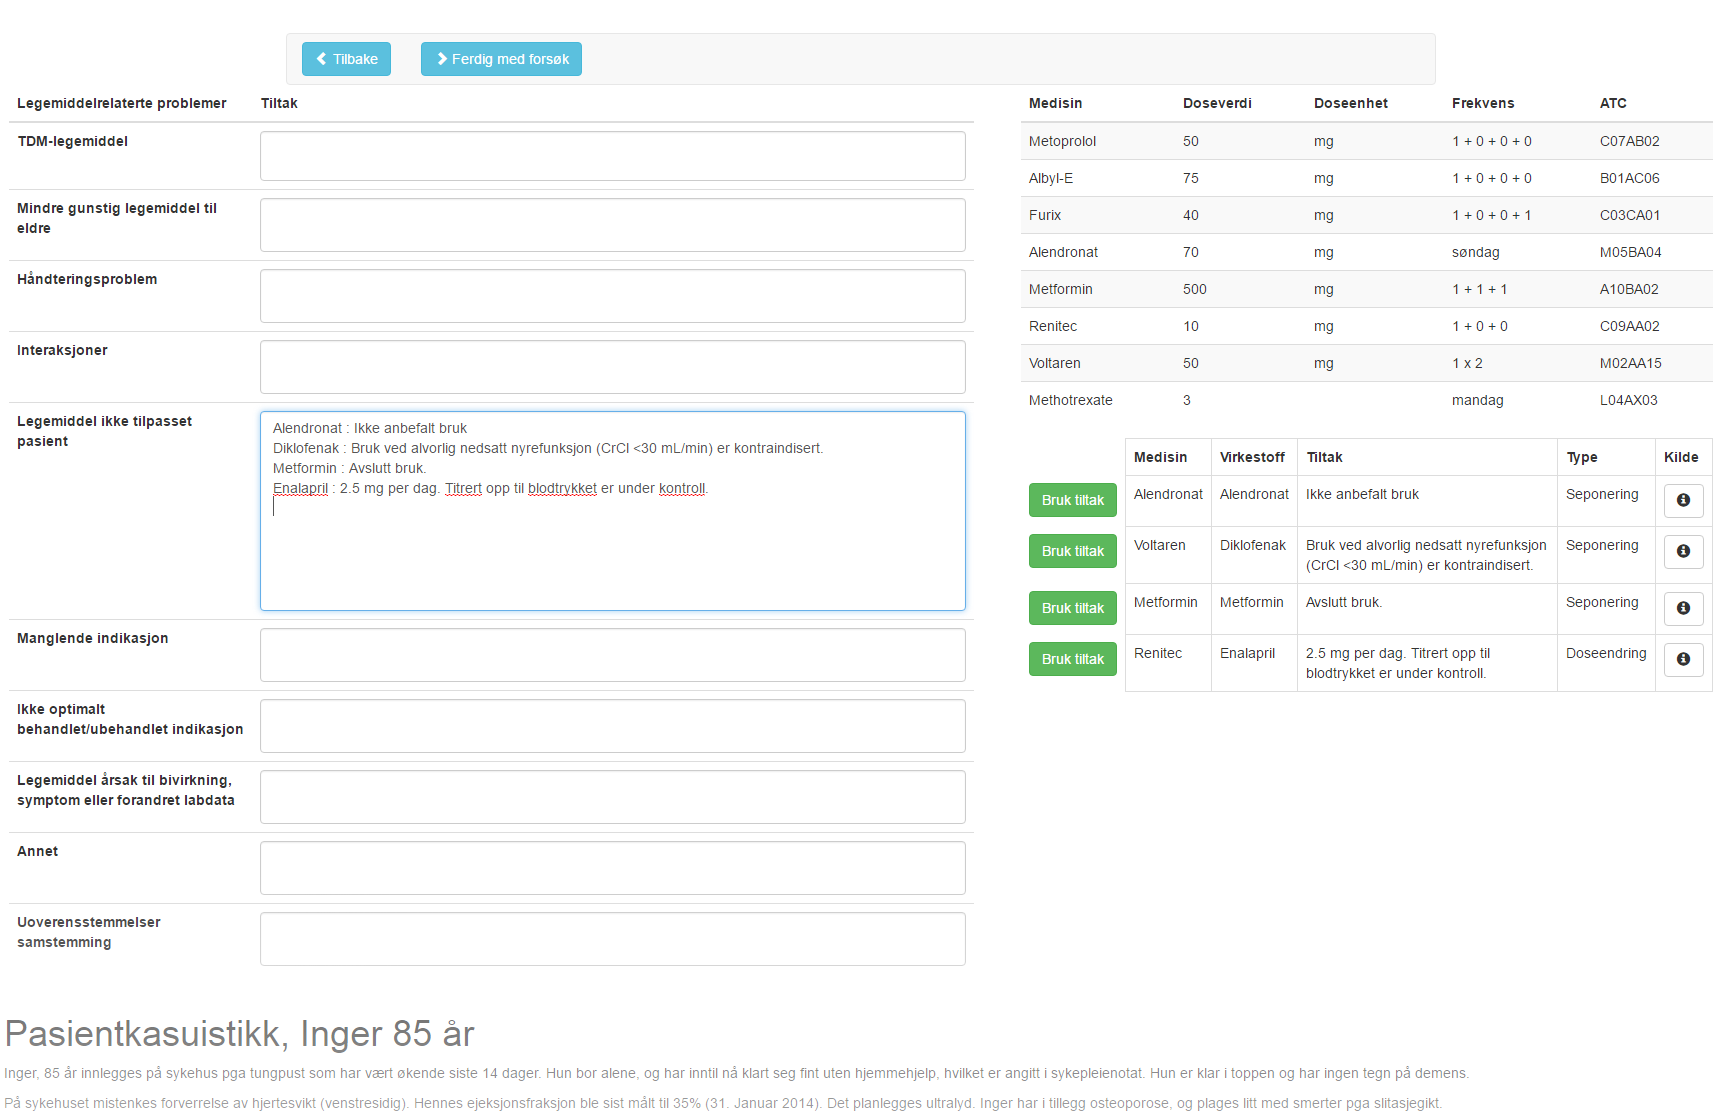
\includegraphics[width=18cm]{images/demoimages/6}
\caption{LMG-vindu med brukte tiltak}
\label{fig:demo6}
\end{center}
\end{figure}

\newpage



\section{Gjennomføring av eksperiment}
\label{chap:gjenomf_eksperiment}
\subsection{Rekruttering av deltagere}
Ved hjelp av våre biveildere ved Sykehusapoteket i Trondheim rekrutterte vi kliniske farmasøyter til å delta i eksperimentet. 30 kliniske farmasøyter ble kontaktet. Disse jobbet primært ved Sykehusapoteket i Trondheim, med noen innslag av kliniske farmasøyter ved sykehusapoteker i Nord-Trøndelag samt Møre og Romsdal. Ut av disse 30 svarte 10 at de ønsket å delta i eksperimentet. Av disse 10 var 4 kliniske farmasøyter ved Sykehusapoteket i Trondheim. 

For å rekruttere kliniske farmasøyter til utføring av et fokusgruppeintervju, måtte vi ta utgangspunkt i de som allerede har sagt seg villig til å delta i eksperimentet. Siden fokusgruppeintervjuet tok utgangspunkt i bruk av støttesystem som SemLMG, ville rekruttering av kliniske farmasøyter som ikke deltok på eksperimentet være ut av kontekst. De fire kliniske farmasøytene som jobbet i Trondheim ble kontaktet, da de resterende syv av praktiske hensyn ikke var mulig å rekruttere.
//For further notice: hvor mange av disse var villige til å delta i fokusgruppe?

\subsection{Informasjon for gjennomføring}
I forkant fikk deltagerne en introduksjon til SemLMG og hvordan de skulle bruke det for å gjennomføre eksperimentet. Denne informasjonen sendte vi ut sammen med brukernavnene til hver enkelt deltager samt tidsfrist og annen praktisk informasjon. Informasjonsskrivet er i sin helhet vedlagt i \ref{vedlegg:informasjonsskriv}.

\subsection{Spørreskjema}
Et spørreskjema ble utviklet. Denne var basert på spørsmål utviklet av en klinisk farmasøyt som tok utgangspunkt i pasientkasuistikkene i SemLMG. Halvparten av spørsmålene var rettet mot foreslåtte tiltak og den andre halvparten på legemiddelrelatert kompetanse. Den andre halvdelen av spørsmålene gikk på dypere kompetansene rundt legemidlene. De fleste spørsmålene hadde flere svaralternativ som den kliniske farmasøyten sto for. Videre ble en fasit utviklet, som vi brukte for å sette en poengsum for antall riktige i spørreundersøkelsen.

Det var flere valgmuligheter når det kom til å lage spørreundersøkelse på nett. Opprinnelig ble Questback brukt. Questback brukes mye i næringslivet, og siden våre biveiledere hadde tilgang til verktøyet virket dette fornuftig\ot{Er dette relevant?}. Etterhvert skulle det vise seg at Questback var vanskelig å konfigurere, i tillegg til at vi ikke hadde tilgang selv. Derfor valgte vi å ta i bruk Google Forms, noe som vi har hatt kjennskap til før. Spørreundersøkelsen er tilgjengelig i \ref{vedlegg:magne} og \ref{vedlegg:inger}.

\subsection{Pretest}
Før eksperimentet kunne starte var det behov for å utføre en pretest. Dette var en prosess vi sammen med veiledere ønsket å utføre for å kunne oppdage og rette feil. Målet var å forbedre prototypen og spørreskjema hvis det var nødvendig. Pretesten ble utført på hovedveileder og biveiledere. \\
Et annet alternativ vi hadde for å kunne få en enda bedre evaluering av forsøket var å ha en pre-pretest samt en pretest. For å kunne gjennomføre dette måtte vi tatt ut to-tre personer fra deltakergruppen og brukt disse til pretest. En pre-pretest kunne da ha blitt utført med hovedveileder og biveiledere, mens pretesten hadde vært faktiske deltakere. Det var planlagt at en person måtte bruke to til tre dager på å utføre eksperimentet. På lik linje ønsket vi at pretestere også skulle få samme antall dager på å utføre en pretest. Dette vil bety at vi ville utsatt datoen for innsamling av resultater fra eksperiment med to-tre dager. Det ble derfor besluttet at eksperimentet var så godt som det kunne bli på den tiden vi hadde, og at en pretest på tre personer var godt nok for å gjøre nødvendige endringer. \\
Vi fikk gode resultater av pretesten. Noen tilbakemeldinger gikk på endringer i grensesnitt, mens andre gikk direkte på kasuistikken. Generelt fikk vi positive tilbakemeldinger.

\subsubsection{Personvern}



\subsection{Fokusgruppeintervju}